\newpage
\section{Our Experiment}
\subsection{Infrastructure}
\paragraph{}As the experiment's infrastructure we will describe the frameworks used during the implementation. The framework that has been used to implement the item-based algorithm was Apache Spark. Also the ALS algorithm was used from the Apache Spark's MLLib library. The framework is common to infrastructure because Apache Spark can orchestrate the work on multiple machine as well as in one. So the framework is the closest you can get to the infrastructure.

\subsubsection{Apache Spark}
The last decade, analyzing big data is at its peek. Lots of data are produced on daily basis. This means that the need of extracting information from them is raised. 
Lots of frameworks has been used in order to manage and analyze this amount of data. One of the analysis reasons is the need for accurate item recommendations to users. Those items could be movies (e.g. Netflix), music (e.g. Spotify) or products in general(e.g. Amazon). The one of the most popular frameworks that could enable this in a distributed way was Apache's Hadoop MapReduce.


Apache Hadoop has also discrete jobs of processing data. The most common jobs are map and reduce but it has two more jobs, combine and partition. Hadoop has a master node and N worker nodes. The first is responsible to distribute the work, and the second for the work to be done. Each worker usually is called after the job is executing. Hence we have the mapper, the reducer, the partitioner and the combiner.
To put this to a schema, you can see the figure \ref{hadoopJobsOrder} below.

\begin{figure}[h]
	\centering
	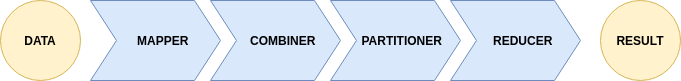
\includegraphics[width=0.5\textwidth]{images/HadoopMapReduceProcesses.png}
	\caption{\bfseries Hadoop Jobs Order}
	\label{hadoopJobsOrder}
\end{figure}

 Hadoop map reduce, is a distributed map-reduce system, 
this means that it has a mechanism to distribute work on nodes 
and a common interface for handling data. In Hadoop's case this was able to happen due to Apache Hadoop Yarn and the Hadoop Distributed File System or as commonly used HDFS.
 When a job was scheduled, data were loaded by the HDFS to a worker, 
then the worker was done, he was putting the result back to the HDFS. 

As mentioned in \cite{ibmMapReduce:5}, "The term MapReduce actually refers to two separate and distinct tasks that Hadoop programs perform. The first is the map job, which takes a set of data and converts it into another set of data, where individual elements are broken down into tuples (key/value pairs). The reduce job takes the output from a map as input and combines those data tuples into a smaller set of tuples. As the sequence of the name MapReduce implies, the reduce job is always performed after the map job."

So Hadoop has two basic processes, Map which is responsible for turning the data into key value pairs, and Reduce which takes those pairs and turns them into valuable data.

If we would like to see where in the DIKW (Data Information Knowledge Wisdom) stack. The Map process would with data and the reduce will end up with information.

Of course this in not always the case, like we said above 
\paragraph{TODO:} remember to mention above
a recommender system would take more than one MapReduce cycles.
 
\begin{figure}[h]
	\centering
	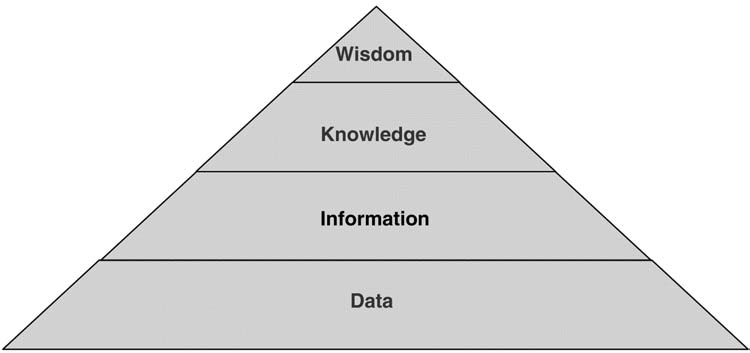
\includegraphics[width=0.5\textwidth]{images/DIKW.png}
	\caption{\bfseries Data Information Knowledge Wisdom Pyramid \cite{TheWisdomHierachy:7}}
	\label{dikw}
\end{figure}
% %note spark version
\paragraph{} But lets make a step back and take a look at Hadoop's architecture. As it is described in its official website \cite{Hadoop:9}, and shown in the figure \ref{hadoopStack} Hadoop uses Hadoop yarn in order to coordinate which process will run on which machine. Also it uses, its filesystem, the HDFS in order to have a common reference for the files over the network. Last but not least, Hadoop ecosystem is supported by the Hadoop Commons library. 

\begin{figure}[h]
	\centering
	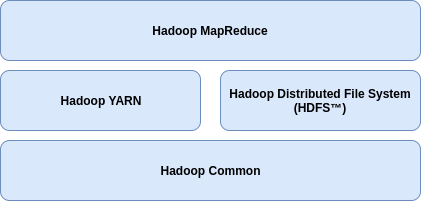
\includegraphics[width=0.5\textwidth]{images/hadoop-stack.png}
	\caption{\bfseries Hadoup Software Stack}
	\label{hadoopStack}
\end{figure}


 In 2009 UC Berkley developed spark \cite{DatabricsSpark:8}. \paragraph{TODO:} Update citation

\paragraph{}Apache spark is the new trend on distributed computation and map-reduce. 
But first things first, what is map-reduce? \\
apache mesos -> data center operating system, references
\\
But innovation knocked the door and resilient distributed datasets entered the room. In spark world, data are loaded to HDFS as before. Then spark loads them in an RDD, this means that data are now accessible on each machine's memory. Any transformation done to a RDD results a RDD, and so forth. After all the transformations are done, spark can transform the results to a file in HDFS.

\begin{figure}[ht]
  \centering
    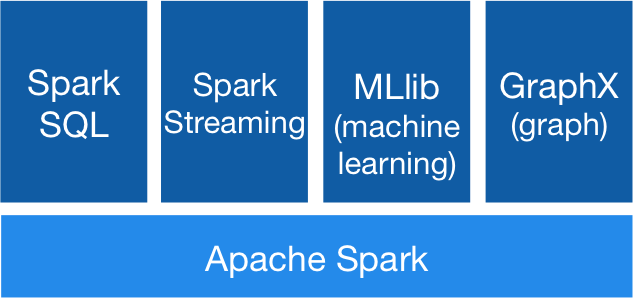
\includegraphics[width=0.5\textwidth]{images/spark-stack.png}
    \caption{\bfseries Apache spark stack \cite{ApacheSpark:1}}
   \label{apacheSparkStack}
\end{figure}


\paragraph{TODO:} Like Hadoop, Spark also follow the structure of master-worker. But unlike Hadoop, Spark has functions that can be distributed. To make things clearer, in spark we can have a map job and the result can be the input to another map job, whereas in Hadoop we couldn't do this.

\paragraph{}
Apache Spark was by design meant to work within Hadoop ecosystem, and most improtanly with the HDFS. Apache Spark does not has a file system by itself. This means that it has to load files from some source. Initially this source was HDFS but Spark has integration with more sources than HDFS. You can load data from almost any database, cloud-based or not, even from a local file system. But most will agree that Hadoop and Spark work together just perfect.

\paragraph{} Once the data are loaded to spark, they are in a structure called RDD (Resilient Distributed Datasets). Those data sets live on disk and on memory. By this you can see that the speed of processing data on Apache Spark it could be much more faster than its predecessor Hadoop map-reduce. 

\paragraph{TODO:} cite a benchmark between hadoop map reduce and apache spark

\paragraph{}
How spark differentiates from its predecessors\\
Spark lightweight in memory data transformation 
Resilient Distributed Datasets (RDDs) \\
mllibs\\
add spark jira note \\\\
Important note: mention als distributed broadcasting implementation. 
\\\\
When a RDD is been broadcasted in Apache Spark, this RDD becomes a local matrix to each machine. This means that you can use it for local calculations. This adds an overload to each machine depending on RDD's size. But it eliminates the network usage.
//cite the mastering apache spark book
\cite{ApacheSpark:1} \\
a Spark cluster to be created on AWS EC2 storage.\\
New trends on spark https://github.com/apache-spark-on-k8s/spark cite this repository too.
\subsection{Dataset}
What is the dataset about. This dataset contains users, movies and the rating user made about the movies.
This dataset is splited to multiple subsets of 80000 training sets and respective 20000 reviews.
This dataset has been used by the related work on .....
\cite{MovieLens:3}

\subsection{Implementation and assumptions}
During the implementation I had to make some assumptions and choices. The first of choices was the framework and the programming language that the implementation would take place. The framework that has been chosen, as you may had already figured out, is apache spark due to its trend and the high scalability it offers. The language of choice was scala, due to its functional nature.
\subsection{Metrics}
After the implementation I had to make the choice of the metrics I was going to use.
\subsubsection{Mean Absolute Error}
As metrics are commonly used the MSE, RMSE and MAE. Due to the fact that the author prefers the last one, MAE was used in this experiment.
\begin{equation}
MAE = \frac{\sum_{i=1}^{n}{|y_{i}-x_{i}|} }{n} = \frac{\sum_{i=1}^{n}\sqrt{{(y_{i}-x_{i})}^{2}}}{n}
\end{equation}
\subsubsection{Execution Time}
Time is measured in milliseconds.
Execution time is always a measure when we are comparing algorithms. 
Even more if those algorithms execution time is heavily dependent to their complexity and not their resources.
